% !TeX root = syllabus_ELEC0053.tex
% !TeX encoding = ISO-8859-1
% !TeX spellcheck = fr_FR

\section{Exercices non r�solus}
\begin{exercise}{}
On consid�re le quadrip�le suivant.
\begin{center}
	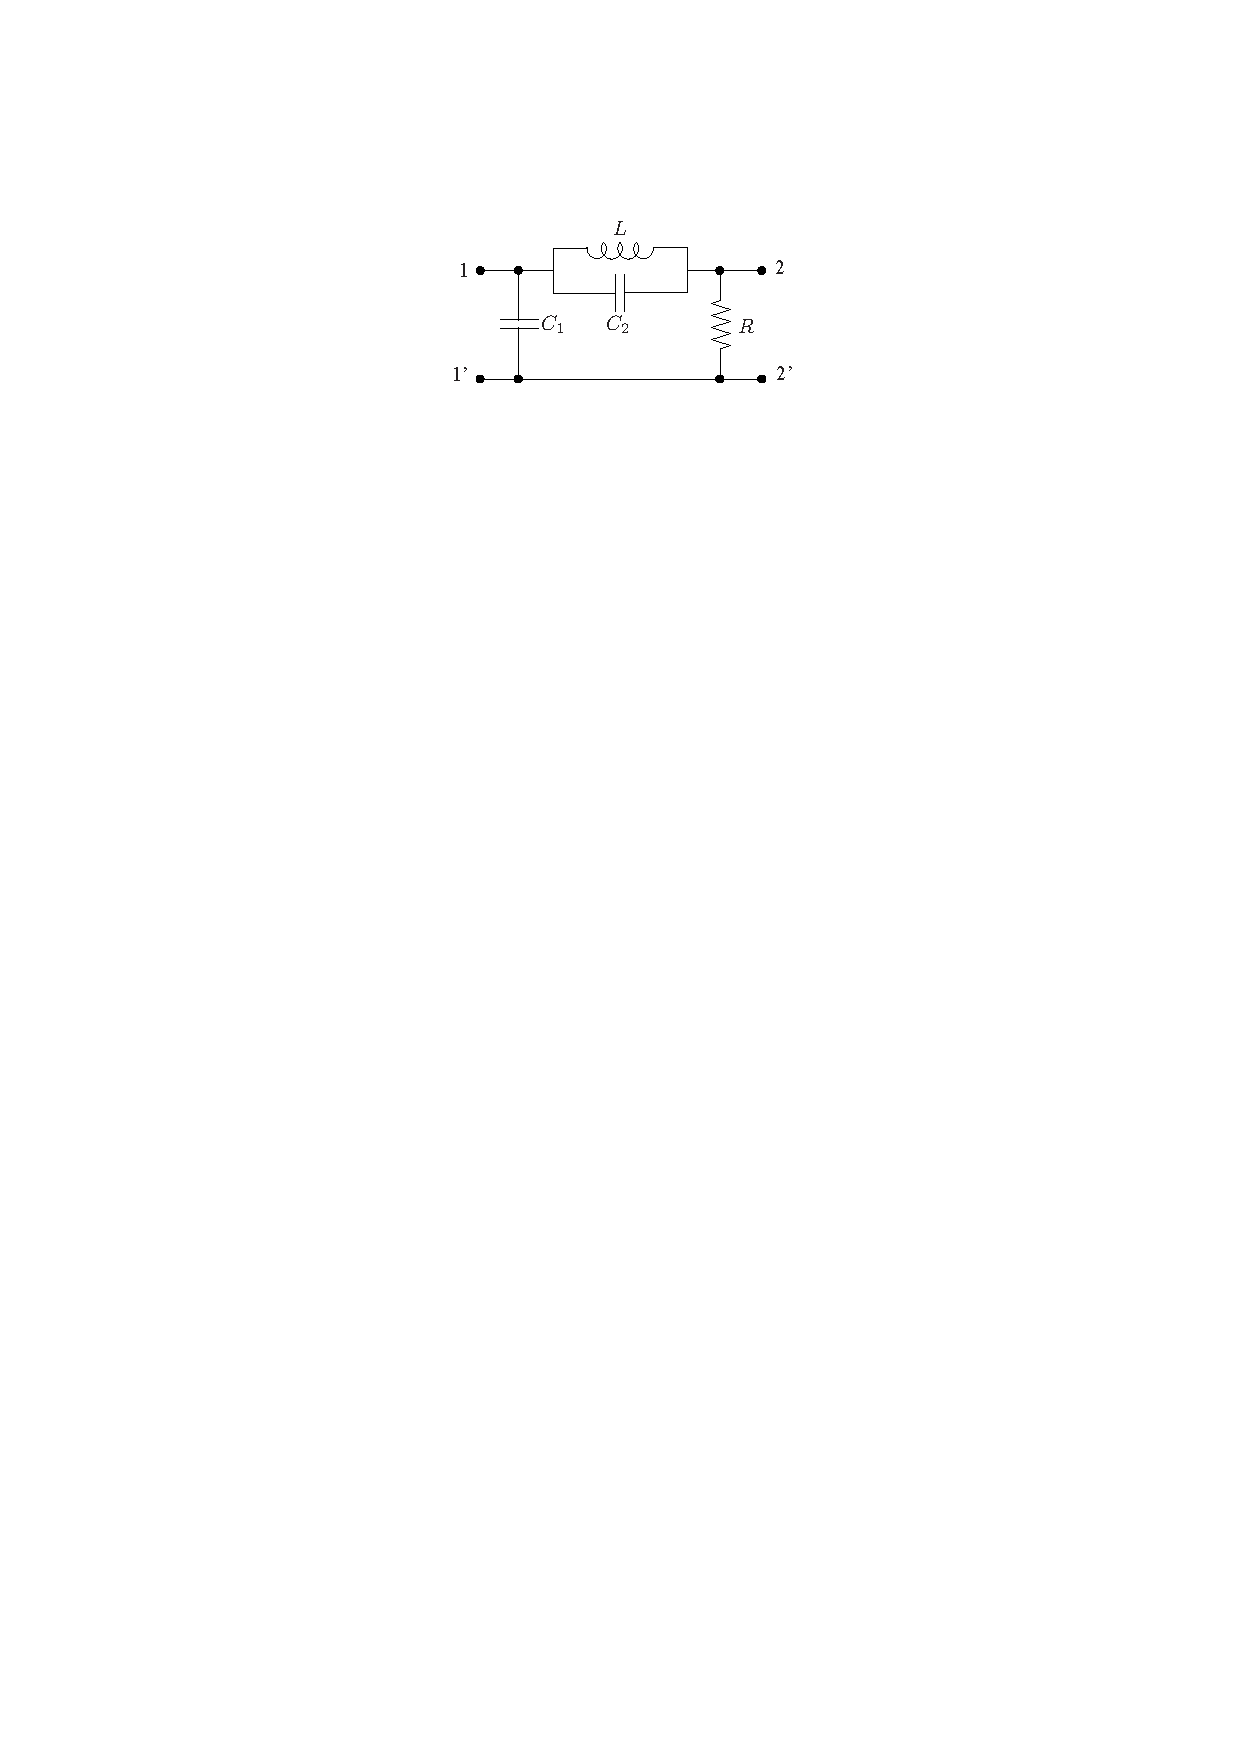
\includegraphics[width=0.5\textwidth]{exercices/ex-4-6} \\
	$C_1=15$ nF ; $C_2=5$ nF ; $L=0.1$ mH ; $R = \frac{400}{3} \Omega$ 
\end{center}
D�terminer:
\begin{enumerate}
	\item la r�ponse fr�quentielle 
	\[H(j\omega)=\left.\frac{\bar{U}_2}{\bar{I}_1}\right|_{\bar{I}_2=0}\]
	\item ses fr�quences naturelles et z�ros de transmission.
\end{enumerate}
\rep{
	$H(j\omega)= \frac{-\omega^2+2\, 10^{12}}{15\, 10^{-9}\left(
		-j\omega^3 - 2\, 10^6\, \omega^2 + 2\, 10^{12} \, j\omega + 10^{18}\right)}$
}
\end{exercise}